\begin{problem}{Romantic Renovation Rescue}{standard input}{standard output}{3 seconds}{1024 megabytes}

Vishwas was planning a surprise for his 6-month relationship anniversary --- a romantic treasure hunt across their college campus. Each stop had sentimental value: the bench where they first talked, the library where they exchanged notes, and their favorite corner in the canteen.

Just days before the big event, the campus was struck by sudden renovations. Many key locations were unexpectedly blocked off, and Vishwas was on the verge of giving up.

That's when Kanav, his best friend and problem-solving genius, stepped in to help. He modeled the entire campus as a weighted undirected graph, where:

 Each node represents a location.
\begin{itemize}
\item Each edge represents a direct path between locations with a positive travel time (weight).
\item Each location can either be open (.) or blocked (x) due to construction.
\end{itemize}

Kanav implemented a system that supports two types of dynamic operations:
\begin{itemize}
\item 0 - Path Query: Given two nodes, determine the shortest path between them using only currently unblocked locations.
\item 1 - Toggle Operation: Toggle the status of a location between blocked and unblocked.
\end{itemize}

Your task is to help Kanav power Vishwas's plan by implementing this dynamic system.

\InputFile
The first line contains a single integer $t$ --- the number of test cases.
$(1 \le t \le 10)$

Each test case consists of the following:

The first line contains three integers $n$, $m$, and $q$ --- the number of nodes, edges, and queries, respectively.
$(2 \le n  \le 1000,\ 1 \le m \le 1000,\ 1 \le q \le 10^4)$

The next $m$ lines each contain three integers $u$, $v$, and $w$ --- representing an undirected edge between nodes $u$ and $v$ with weight $w$.
$(1 \le u, v \le n,\ 1 \le w \le 10^9)$

The next line contains a string of length $n$ consisting only of characters `.' and `x', representing the initial status of each location (`.' indicates that the location is open) and (`x' indicates that the location is blocked).

The next $q$ lines each contain a query starting with $a_i\ $--- where:

\begin{itemize}
\item If $a_i = 0$, the format of query is $a_i\ x_i\ y_i$ --- it is a path query: compute the shortest path from node $x_i$ to node $y_i$ using only unblocked nodes.

\item If $a_i = 1$, the format of query is $a_i\ x_i\ $ --- it is a toggle operation: toggle the blocked/unblocked status of node $x_i$. 
\end{itemize}

\textbf{Note}:
\begin{itemize}
\item The sum of $n \times m$ over all test cases does not exceed $10^6$.

\item For each test case, the total sum of $a_i$ over all queries is at most $10$.

\item In the string `.' is the dot or fullstop in english keyboard and `x' is the alphabetic character x.
\end{itemize}

\OutputFile
For each query of type 0 x y, print the minimum total time (sum of edge weights) from node
x to node y using only unblocked nodes. If no path exists, print -1.

Note: If x and y are same nodes output 0. And if either one of them is blocked then output -1.

\Examples

\begin{example}
\exmpfile{example.01}{example.01.a}%
\exmpfile{example.02}{example.02.a}%
\end{example}

\Note
For \textbf{first} example, it given that there are total 4 nodes and 5 edges. Then next 5 lines represent 5 weighted edges.

Also in the string ``..x.", it is given that Node 3 is blocked initially, hence graph will look like this.
\begin{center}
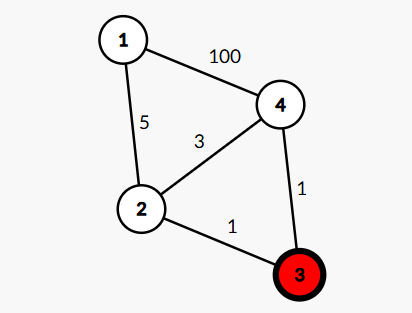
\includegraphics{q1-graph.png}
\end{center}
Orignally path 1, 2, 4 is taken which costs $ 5 + 3 = 8 $ while once Node 3 is toggled (and hence unblocked) path 1, 2, 3, 4 is taken which costs $ 5 + 1 + 1 = 7 $.

Similarly for the \textbf{second} example graph goes as follows after each toggle.
\begin{center}
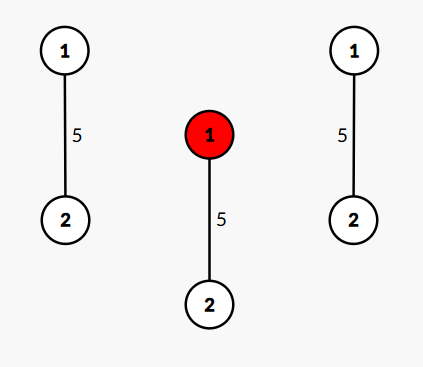
\includegraphics{q2-graph.png}
\end{center}
Initially 
\begin{itemize}
\item 1 to 2 is possible and cost is 5.
\item 1 to 1 is possible and cost is 0.
\item 2 to 2 is possible and cost is 0.
\end{itemize}
After blocking Node 1:
\begin{itemize}
\item 1 to 2 is not possible and hence print -1. (Since 1 is blocked)
\item 1 to 1 is not possible and hence print -1. (Since 1 is blocked)
\item 2 to 2 is possible and cost is 0.
\end{itemize}

\end{problem}

